\section{Arrays}

\begin{frame}
	\centering
	\Huge \textbf{Arrays}
\end{frame}

%\subsection{What is an Array?}

\begin{frame}[fragile]{Arrays in Fortran}
  \begin{columns}[T]

    \column{0.55\textwidth}
    \begin{block}{Idea}
      Arrays (vectors, matrices, tensors) hold multiple values of the same type.
      Elements are accessed by subscripts.
    \end{block}

    \begin{block}{Examples (declarations)}
      \texttt{real, dimension(6) :: X}\\
      \texttt{real, dimension(1:5,1:3) :: Y}
    \end{block}

    \begin{block}{Every array has}
      Type (e.g., real), a rank (number of dimensions), bounds for each dimension,
      and a value for each element.
    \end{block}

    \column{0.45\textwidth}
    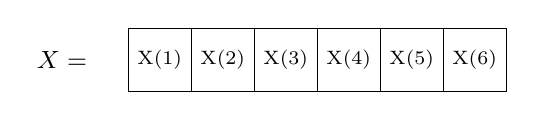
\begin{tikzpicture}[
      cell/.style={draw, minimum width=0.8cm, minimum height=0.8cm, font=\scriptsize}
    ]
      \node[anchor=east,font=\small] (arr1) at (0,0) {$X =$};
      \foreach \i in {1,...,6} {
        \node[cell] (x\i) at (\i*0.8,0) {X(\i)};
      }
    \end{tikzpicture}

    \vspace{0.8cm}

    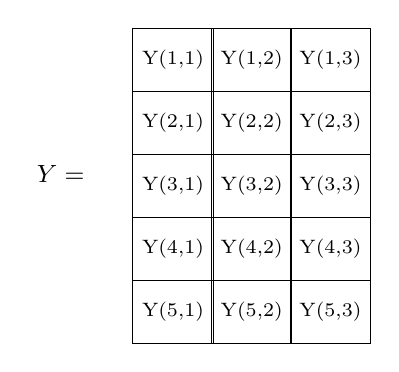
\begin{tikzpicture}[
      cell/.style={draw, minimum width=1.0cm, minimum height=0.8cm, font=\scriptsize}
    ]
      \node[anchor=east,font=\small] (arr2) at (0,-2.25) {$Y =$};
      \foreach \i in {1,...,5}{
        \foreach \j in {1,...,3}{
          \pgfmathtruncatemacro{\yy}{4-\j}
          \node[cell] at (\j,-\i*0.8) {Y(\i,\j)};
        }
      }
    \end{tikzpicture}

  \end{columns}
\end{frame}


\begin{frame}{Array Terminology}
  \begin{block}{Definitions}
    \begin{itemize}
      \item \textbf{Rank}: number of dimensions (e.g., 1D, 2D).
      \item \textbf{Bounds}: lower/upper index limits in each dimension.
      \item \textbf{Extent}: number of elements along a dimension.
      \item \textbf{Size}: total number of elements.
      \item \textbf{Shape}: tuple of extents.
      \item \textbf{Conformable}: same shape (element-wise operations valid).
    \end{itemize}
  \end{block}
  \begin{block}{Examples}
    With \texttt{real, dimension(15) :: X} and \texttt{real, dimension(1:5,1:3) :: Y}:\\
    rank(X)=1; bounds(X)=1:15; extent(X)=15; size(X)=15; shape(X)=(/15/).\\
    Y and Z: rank=2; shape=(/5,3/); they are conformable.
  \end{block}
\end{frame}

%\subsection{Declaring Arrays}

\begin{frame}{Explicit-Shape Declarations}
  \begin{block}{Forms}
    \begin{itemize}
      \item \texttt{real, dimension(100) :: R}
      \item \texttt{real, dimension(1:10,1:10) :: S}
      \item \texttt{real :: T(10,10)}
      \item \texttt{real, dimension(-10:-1) :: X}
      \item \texttt{integer, parameter :: lda = 5}\\
            \texttt{real, dimension(0:lda-1) :: Y}
      \item \texttt{real, dimension(1+lda*lda,10) :: Z}
    \end{itemize}
  \end{block}
  \begin{block}{Notes}
    Default lower bound is 1; bounds may begin/end anywhere; arrays can be zero-sized if bounds imply size 0.
  \end{block}
\end{frame}

%\subsection{Conformance and Ordering}

\begin{frame}{Conformance Rules}
  \begin{block}{Element-wise operations}
    Arrays (or sections) in an expression must conform (same shape). A scalar conforms with any shape.
  \end{block}
  \begin{block}{Examples}
    \texttt{C = 1.0} (broadcasts to all elements) — valid.\\
    \texttt{C = D} (same shape) — valid.\\
    \texttt{B = A} (same size but different shape) — invalid.
  \end{block}
\end{frame}

\begin{frame}{Array Element Ordering}
  \begin{block}{Conceptual order}
    Fortran defines a column-major element order for intrinsic operations and I/O:\\
    \texttt{C(1,1), C(2,1), ..., C(n,1), C(1,2), ..., C(n,m)}
  \end{block}
  \begin{block}{Storage}
    The standard does not mandate physical memory layout beyond this conceptual ordering; avoid relying on storage association.
  \end{block}
\end{frame}

%\subsection{Array Syntax and Sections}


\begin{frame}[fragile]{Subscript Triplets}
	\begin{block}{General form}
		\texttt{[lb]:[ub][:stride]} with scalar integer expressions. Examples:
	\end{block}
	\begin{block}{Examples}
		\begin{lstlisting}[language=Fortran]
		A(:)        ! whole array
		A(3:9)      ! A(3) .. A(9) step 1
		A(3:9:1)    ! same as above
		A(m:n)      ! lower/upper bounds
		A(m:n:k)    ! step k
		A(8:3:-1)   ! descending section
		A(8:3)      ! zero-sized (default step 1)
		A(m:)       ! m .. upper bound
		A(:n)       ! lower bound .. n
		A(::2)      ! every 2nd element
		A(m:m)      ! 1-element section
		A(m)        ! scalar element (not a section)
		\end{lstlisting}
	\end{block}
\end{frame}


\begin{frame}[fragile]{Whole Arrays, Elements, and Sections}
  \begin{block}{Whole arrays}
\begin{lstlisting}[language=Fortran]
A = 0.0             ! set every element of A to zero
B = C + D           ! element-wise add C and D into B
\end{lstlisting}
  \end{block}
  \begin{block}{Elements}
\begin{lstlisting}[language=Fortran]
A(1) = 0.0
B(0,0) = A(3) + C(5,1)
\end{lstlisting}
  \end{block}
  \begin{block}{Sections}
\begin{lstlisting}[language=Fortran]
A(2:4) = 0.0
B(-1:0,1:2) = C(1:2,2:3) + 1.0
\end{lstlisting}
  \end{block}
\end{frame}

\begin{frame}[fragile]{Whole-Array Expressions}
  \begin{block}{Elemental semantics}
    Intrinsic operators/functions act element-wise on conformable arrays.
  \end{block}
  \begin{block}{Examples}
\begin{lstlisting}[language=Fortran]
B = C * D - B**2    ! element-wise
B = sin(C) + cos(D) ! elemental intrinsics
\end{lstlisting}
  \end{block}
\end{frame}

%\begin{frame}{Section Visualisation and Validity}
%  \begin{block}{Given}
%    \texttt{real, dimension(1:6,1:8) :: P}
%  \end{block}
%  \begin{block}{Valid}
%    \texttt{P(1:3,1:4) = P(1:6:2,1:8:2)}\\
%    \texttt{P(1:3,1:4) = 1.0}
%  \end{block}
%  \begin{block}{Invalid}
%    \texttt{P(2:8:2,1:7:3) = P(1:3,1:4)} (shapes differ)\\
%    \texttt{P(2:6:2,1:7:3) = P(2:5,7)} (1D section vs 2D section)
%  \end{block}
%\end{frame}

\begin{frame}[fragile]{Array Indexing: Single Element}
  \begin{columns}[T]
    \column{0.45\textwidth}
    \begin{block}{Indexing Example}
      \texttt{A(3,4)} \\
      \vspace{0.5em}
      Selects one element at row \texttt{3}, column \texttt{4}.
    \end{block}
    \begin{block}{Array Shape}
      \texttt{A(1:5, 1:5)} (5x5)
    \end{block}

    \column{0.55\textwidth}
    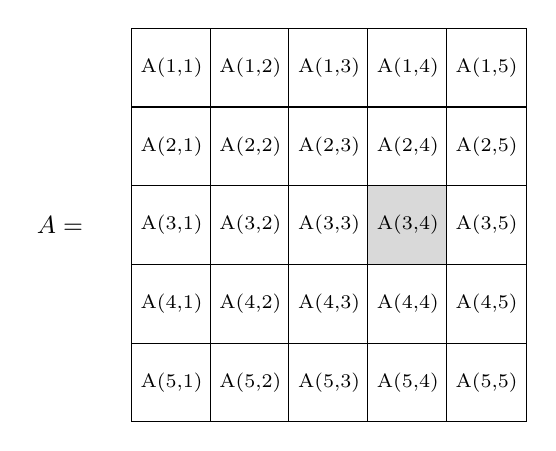
\begin{tikzpicture}[
      x=1cm, y=1cm,
      cell/.style={draw, minimum width=1cm, minimum height=1cm,
                   font=\scriptsize, text=black}
    ]
      \node[anchor=east,font=\small] at (0,-3) {$A =$};
      \foreach \i in {1,...,5} {
        \foreach \j in {1,...,5} {
          \pgfmathtruncatemacro{\yy}{-\i}
          \def\fillopt{white}
          \ifnum\i=3\relax
            \ifnum\j=4\relax
              \def\fillopt{gray!30}
            \fi
          \fi
          \node[cell,fill=\fillopt] at (\j,\yy) {A(\i,\j)};
        }
      }
    \end{tikzpicture}
  \end{columns}
\end{frame}

\begin{frame}[fragile]{Array Indexing: Row Section}
  \begin{columns}[T]
    \column{0.45\textwidth}
    \begin{block}{Indexing Example}
      \texttt{A(2,:)}\\[0.5em]
      Selects all columns on row \texttt{2}.
    \end{block}
    \begin{block}{Array Shape}
      \texttt{A(1:5, 1:5)} (5x5)
    \end{block}

    \column{0.55\textwidth}
    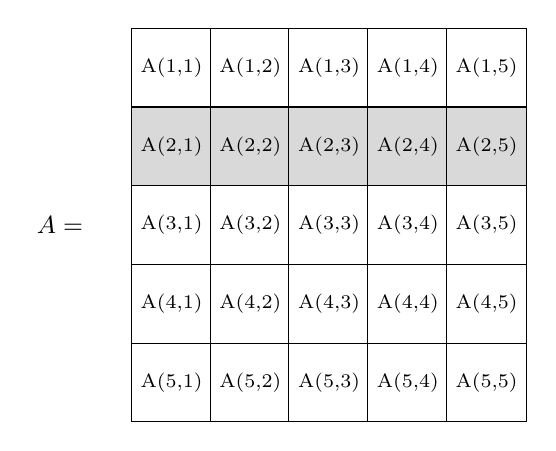
\begin{tikzpicture}[
      x=1cm, y=1cm,
      cell/.style={draw, minimum width=1cm, minimum height=1cm,
                   font=\scriptsize, align=center, text=black}
    ]
      \node[anchor=east,font=\small] at (0,-3) {$A =$};
      \foreach \i in {1,...,5} {
        \foreach \j in {1,...,5} {
          \pgfmathtruncatemacro{\yy}{-\i}
          \def\fillopt{white}
          \ifnum\i=2\relax
            \def\fillopt{gray!30}
          \fi
          \node[cell,fill=\fillopt] at (\j,\yy) {A(\i,\j)};
        }
      }
    \end{tikzpicture}
  \end{columns}
\end{frame}

\begin{frame}[fragile]{Array Indexing: Column Section}
  \begin{columns}[T]
    \column{0.45\textwidth}
    \begin{block}{Indexing Example}
      \texttt{A(:,3)}\\[0.5em]
      Selects all rows in column \texttt{3}.
    \end{block}
    \begin{block}{Array Shape}
      \texttt{A(1:5, 1:5)} (5x5)
    \end{block}

    \column{0.55\textwidth}
    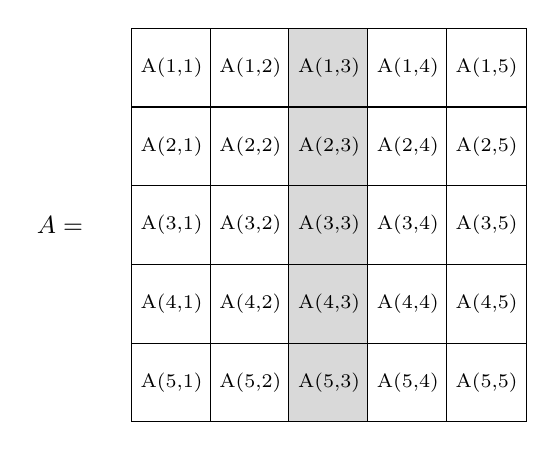
\begin{tikzpicture}[
      x=1.0cm, y=1.0cm,
      cell/.style={draw, minimum width=1.0cm, minimum height=1.0cm,
                   font=\scriptsize, align=center, text=black}
    ]
      \node[anchor=east,font=\small] at (0,-3) {$A =$};
      \foreach \i in {1,...,5} {
        \foreach \j in {1,...,5} {
          \pgfmathtruncatemacro{\yy}{-\i}
          \def\fillopt{white}
          \ifnum\j=3\relax
            \def\fillopt{gray!30}
          \fi
          \node[cell,fill=\fillopt] at (\j,\yy) {A(\i,\j)};
        }
      }
    \end{tikzpicture}
  \end{columns}
\end{frame}

\begin{frame}[fragile]{Array Indexing: Subarray}
  \begin{columns}[T]
    \column{0.45\textwidth}
    \begin{block}{Indexing Example}
      \texttt{A(2:4, 2:5)}\\[0.5em]
      Selects rows 2–4 and columns 2–5 (a 3x4 block).
    \end{block}
    \begin{block}{Array Shape}
      \texttt{A(1:5, 1:5)} (5x5)
    \end{block}

    \column{0.55\textwidth}
    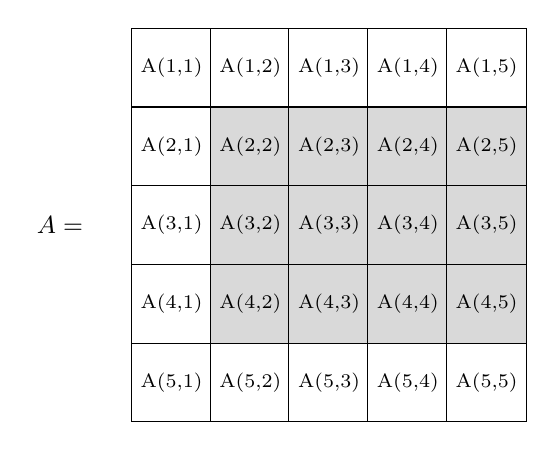
\begin{tikzpicture}[
      x=1.0cm, y=1.0cm,
      cell/.style={draw, minimum width=1.0cm, minimum height=1.0cm,
                   font=\scriptsize, align=center, text=black}
    ]
      \node[anchor=east,font=\small] at (0,-3) {$A =$};
      \foreach \i in {1,...,5} {
        \foreach \j in {1,...,5} {
          \pgfmathtruncatemacro{\yy}{-\i}
          \def\fillopt{white}
          % Subarray highlight
          \ifnum\i>1\relax\ifnum\i<5\relax
            \ifnum\j>1\relax
              \def\fillopt{gray!30}
            \fi
          \fi\fi
          \node[cell,fill=\fillopt] at (\j,\yy) {A(\i,\j)};
        }
      }
    \end{tikzpicture}
  \end{columns}
\end{frame}

\begin{frame}[fragile]{Array Indexing: Strided Selection}
  \begin{columns}[T]
    \column{0.45\textwidth}
    \begin{block}{Indexing Example}
      \texttt{A(1:5:2, 2:5:2)}\\[0.5em]
      Selects odd rows and even columns.
    \end{block}
    \begin{block}{Array Shape}
      \texttt{A(1:5, 1:5)} (5x5)
    \end{block}

    \column{0.55\textwidth}
    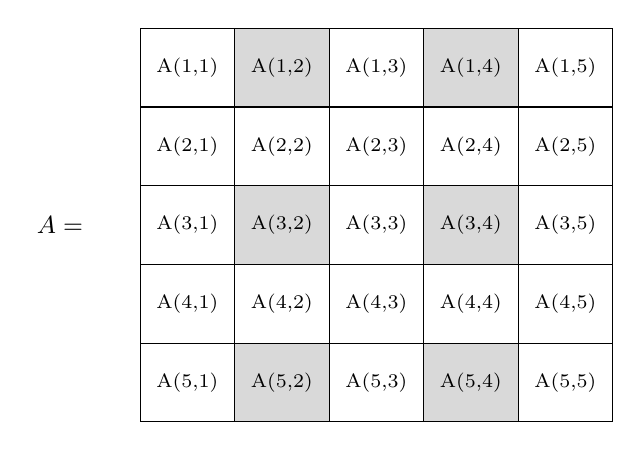
\begin{tikzpicture}[
      x=1.2cm, y=1.0cm,
      cell/.style={draw, minimum width=1.2cm, minimum height=1.0cm,
                   font=\scriptsize, align=center, text=black}
    ]
      \node[anchor=east,font=\small] at (0,-3) {$A =$};
      \foreach \i in {1,...,5} {
        \foreach \j in {1,...,5} {
          \pgfmathtruncatemacro{\yy}{-\i}
          \def\fillopt{white}
          % Strided highlight: odd i, even j
          \ifodd\i
            \ifodd\j\else
              \def\fillopt{gray!30}
            \fi
          \fi
          \node[cell,fill=\fillopt] at (\j*1,\yy) {A(\i,\j)};
        }
      }
    \end{tikzpicture}
  \end{columns}
\end{frame}


%\subsection{Array I/O}

\begin{frame}{Array I/O Ordering}
  \begin{block}{print*, A}
    Outputs elements in column-major order: \texttt{A(1,1), A(2,1), ..., A(1,2), ...}
  \end{block}
  \begin{block}{read*, A}
    Reads elements in the same conceptual order. Use \texttt{reshape}, \texttt{transpose}, \texttt{cshift} to alter layout or view.
  \end{block}
\end{frame}

\begin{frame}[fragile]{Array I/O Example}
\begin{block}{Program}
\begin{lstlisting}[language=Fortran]
program Owt
  implicit none
  integer, parameter :: n=3
  integer :: a(n,n)
  a = reshape((/1,2,3,4,5,6,7,8,9/), (/n,n/))
  print*, 'Element =', a(3,2)
  print*, 'Column 1 =', a(:,1)
  print*, 'Subarray =', a(:2,:2)
  print*, 'Whole   =', a
  print*, 'Transposed =', transpose(a)
end program Owt
\end{lstlisting}
\end{block}
\end{frame}

%\section{Allocatable Arrays}
%
%\begin{frame}[fragile]{Deferred-Shape (Allocatable) Arrays}
%  \begin{block}{Declaration}
%\begin{lstlisting}[language=Fortran]
%integer, dimension(:),   ALLOCATABLE :: ages   ! 1D
%real,    dimension(:,:), ALLOCATABLE :: speed  ! 2D
%\end{lstlisting}
%  \end{block}
%  \begin{block}{Allocation}
%\begin{lstlisting}[language=Fortran]
%integer :: isize, ierr
%READ*, isize
%ALLOCATE(ages(isize), STAT=ierr)
%IF (ierr /= 0) print*, 'ages: allocation failed'
%ALLOCATE(speed(0:isize-1,10), STAT=ierr)
%IF (ierr /= 0) print*, 'speed: allocation failed'
%\end{lstlisting}
%  \end{block}
%  \begin{block}{Note}
%    \texttt{STAT=} is optional but recommended to detect errors.
%  \end{block}
%\end{frame}
%
%\begin{frame}[fragile]{Deallocation and Status}
%  \begin{block}{Deallocate}
%\begin{lstlisting}[language=Fortran]
%integer :: ierr
%IF (ALLOCATED(ages)) DEALLOCATE(ages, STAT=ierr)
%IF (ALLOCATED(speed)) DEALLOCATE(speed, STAT=ierr)
%\end{lstlisting}
%  \end{block}
%  \begin{block}{Guidelines}
%    \begin{itemize}
%      \item Only deallocate allocatable arrays that are currently allocated.
%      \item Prefer checking \texttt{ALLOCATED(array)} before deallocation.
%      \item In procedures, deallocate before exit unless the array has \texttt{SAVE}.
%    \end{itemize}
%  \end{block}
%\end{frame}

%\subsection{Wrap-up}

\begin{frame}{Key Takeaways}
  \begin{block}{Summary}
    \begin{itemize}
      \item Know rank, bounds, shape, size; ensure conformance in expressions.
      \item Use whole-array assignments and elemental intrinsics idiomatically.
      \item Master sections with subscript triplets; watch out for zero-sized sections.
      \item Understand column-major ordering for I/O.
      %\item Use allocatable arrays with \texttt{ALLOCATE}/\texttt{DEALLOCATE} and \texttt{STAT=}.
    \end{itemize}
  \end{block}
\end{frame}

\section{Exercises}

\begin{frame}[fragile]
	\frametitle{Exercises}
	\begin{columns}[T]
		\begin{column}{0.5\textwidth}
			\textbf{Exercise 1:}
			\begin{itemize}
				\item Write a program that computes and prints the matrix multiplication of two real arrays.
			\end{itemize}
			\vspace*{0.2cm}
			\[
			A = \begin{pmatrix}
			3 & 2 & 4 & 1 \\
			2 & 4 & 2 & 2 \\
			1 & 2 & 3 & 7
			\end{pmatrix}
			\quad
			B = \begin{pmatrix}
			3 & 2 & 4 \\
			2 & 1 & 2 \\
			3 & 0 & 2
			\end{pmatrix}
			\]
		\end{column}
		
		\begin{column}{0.5\textwidth}
			\textbf{Exercise 2:}
			\begin{itemize}
				\item Write a Fortran program that reads an integer from the user and determines whether it is a palindrome (whether its digits read the same forwards and backwards).
			\end{itemize}
			
%			\textbf{Exercise 3:}
%			\begin{itemize}
%				\item Write a program that reads two real arrays of length n and prints the sum of these arrays.
%			\end{itemize}
		\end{column}
	\end{columns}
\end{frame}
